% Template for PLoS
% Version 3.5 March 2018
%
% % % % % % % % % % % % % % % % % % % % % %
%
% -- IMPORTANT NOTE
%
% This template contains comments intended 
% to minimize problems and delays during our production 
% process. Please follow the template instructions
% whenever possible.
%
% % % % % % % % % % % % % % % % % % % % % % % 
%
% Once your paper is accepted for publication, 
% PLEASE REMOVE ALL TRACKED CHANGES in this file 
% and leave only the final text of your manuscript. 
% PLOS recommends the use of latexdiff to track changes during review, as this will help to maintain a clean tex file.
% Visit https://www.ctan.org/pkg/latexdiff?lang=en for info or contact us at latex@plos.org.
%
%
% There are no restrictions on package use within the LaTeX files except that 
% no packages listed in the template may be deleted.
%
% Please do not include colors or graphics in the text.
%
% The manuscript LaTeX source should be contained within a single file (do not use \input, \externaldocument, or similar commands).
%
% % % % % % % % % % % % % % % % % % % % % % %
%
% -- FIGURES AND TABLES
%
% Please include tables/figure captions directly after the paragraph where they are first cited in the text.
%
% DO NOT INCLUDE GRAPHICS IN YOUR MANUSCRIPT
% - Figures should be uploaded separately from your manuscript file. 
% - Figures generated using LaTeX should be extracted and removed from the PDF before submission. 
% - Figures containing multiple panels/subfigures must be combined into one image file before submission.
% For figure citations, please use "Fig" instead of "Figure".
% See http://journals.plos.org/plosone/s/figures for PLOS figure guidelines.
%
% Tables should be cell-based and may not contain:
% - spacing/line breaks within cells to alter layout or alignment
% - do not nest tabular environments (no tabular environments within tabular environments)
% - no graphics or colored text (cell background color/shading OK)
% See http://journals.plos.org/plosone/s/tables for table guidelines.
%
% For tables that exceed the width of the text column, use the adjustwidth environment as illustrated in the example table in text below.
%
% % % % % % % % % % % % % % % % % % % % % % % %
%
% -- EQUATIONS, MATH SYMBOLS, SUBSCRIPTS, AND SUPERSCRIPTS
%
% IMPORTANT
% Below are a few tips to help format your equations and other special characters according to our specifications. For more tips to help reduce the possibility of formatting errors during conversion, please see our LaTeX guidelines at http://journals.plos.org/plosone/s/latex
%
% For inline equations, please be sure to include all portions of an equation in the math environment.  For example, x$^2$ is incorrect; this should be formatted as $x^2$ (or $\mathrm{x}^2$ if the romanized font is desired).
%
% Do not include text that is not math in the math environment. For example, CO2 should be written as CO\textsubscript{2} instead of CO$_2$.
%
% Please add line breaks to long display equations when possible in order to fit size of the column. 
%
% For inline equations, please do not include punctuation (commas, etc) within the math environment unless this is part of the equation.
%
% When adding superscript or subscripts outside of brackets/braces, please group using {}.  For example, change "[U(D,E,\gamma)]^2" to "{[U(D,E,\gamma)]}^2". 
%
% Do not use \cal for caligraphic font.  Instead, use \mathcal{}
%
% % % % % % % % % % % % % % % % % % % % % % % % 
%
% Please contact latex@plos.org with any questions.
%
% % % % % % % % % % % % % % % % % % % % % % % %

\documentclass[10pt,letterpaper]{article}
\usepackage[top=0.85in,left=2.75in,footskip=0.75in]{geometry}

% amsmath and amssymb packages, useful for mathematical formulas and symbols
\usepackage{amsmath,amssymb}

% Use adjustwidth environment to exceed column width (see example table in text)
\usepackage{changepage}

% Use Unicode characters when possible
\usepackage[utf8x]{inputenc}

% textcomp package and marvosym package for additional characters
\usepackage{textcomp,marvosym}

% cite package, to clean up citations in the main text. Do not remove.
\usepackage{cite}

% Use nameref to cite supporting information files (see Supporting Information section for more info)
\usepackage{nameref,hyperref}

% line numbers
\usepackage[right]{lineno}

% ligatures disabled
\usepackage{microtype}
\DisableLigatures[f]{encoding = *, family = * }

% color can be used to apply background shading to table cells only
\usepackage[table,dvipsnames]{xcolor}

% array package and thick rules for tables
\usepackage{array}

%strikethrough
\usepackage{soul}

%sara: for commenting the pdf to add alt text (if anyone knows a better solution for atl text please help)
\usepackage{pdfcomment}

% create "+" rule type for thick vertical lines
\newcolumntype{+}{!{\vrule width 2pt}}

% create \thickcline for thick horizontal lines of variable length
\newlength\savedwidth
\newcommand\thickcline[1]{%
  \noalign{\global\savedwidth\arrayrulewidth\global\arrayrulewidth 2pt}%
  \cline{#1}%
  \noalign{\vskip\arrayrulewidth}%
  \noalign{\global\arrayrulewidth\savedwidth}%
}

% \thickhline command for thick horizontal lines that span the table
\newcommand\thickhline{\noalign{\global\savedwidth\arrayrulewidth\global\arrayrulewidth 2pt}%
\hline
\noalign{\global\arrayrulewidth\savedwidth}}


% Remove comment for double spacing
%\usepackage{setspace} 
%\doublespacing

% Text layout
\raggedright
\setlength{\parindent}{0.5cm}
\textwidth 5.25in 
\textheight 8.75in

% Bold the 'Figure #' in the caption and separate it from the title/caption with a period
% Captions will be left justified
\usepackage[aboveskip=1pt,labelfont=bf,labelsep=period,justification=raggedright,singlelinecheck=off]{caption}
\renewcommand{\figurename}{Fig}

% Use the PLoS provided BiBTeX style
\bibliographystyle{plos2015}

% Remove brackets from numbering in List of References
\makeatletter
\renewcommand{\@biblabel}[1]{\quad#1.}
\makeatother



% Header and Footer with logo
\usepackage{lastpage,fancyhdr,graphicx}
\usepackage{epstopdf}
%\pagestyle{myheadings}
\pagestyle{fancy}
\fancyhf{}
%\setlength{\headheight}{27.023pt}
%\lhead{\includegraphics[width=2.0in]{PLOS-submission.eps}}
\rfoot{\thepage/\pageref{LastPage}}
\renewcommand{\headrulewidth}{0pt}
\renewcommand{\footrule}{\hrule height 2pt \vspace{2mm}}
\fancyheadoffset[L]{2.25in}
\fancyfootoffset[L]{2.25in}
\lfoot{\today}

%% Include all macros below

\newcommand{\lorem}{{\bf LOREM}}
\newcommand{\ipsum}{{\bf IPSUM}}

%% END MACROS SECTION


\begin{document}

\newcommand{\fede}[1]{\textcolor{ForestGreen}{Fede: #1}}
\newcommand{\rocio}[1]{\textcolor{MidnightBlue}{Rocio: #1}}
\newcommand{\doro}[1]{\textcolor{RedViolet}{Dorothea: #1}}
\newcommand{\jani}[1]{\textcolor{YellowOrange}{Janina: #1}}
\newcommand{\la}[1]{\textcolor{RawSienna}{Laura: #1}}
\newcommand{\as}[1]{\textcolor{Violet}{Andrea: #1}}
\newcommand{\rita}[1]{\textcolor{CarnationPink}{Rita: #1}}

\vspace*{0.2in}

% Title must be 250 characters or less.
\begin{flushleft}
{\Large
\textbf\newline{Ten simple rules towards hosting an inclusive conference} % Please use "sentence case" for title and headings (capitalize only the first word in a title (or heading), the first word in a subtitle (or subheading), and any proper nouns).
}
\newline
% Insert author names, affiliations and corresponding author email (do not include titles, positions, or degrees).
\\
Rocío Joo\textsuperscript{1*}, %,2\Yinyang},
Andrea Sánchez-Tapia\textsuperscript{2},
Sara Mortara\textsuperscript{3},
Heather Turner\textsuperscript{4}, %\ddag},
Dorothea Hug Peter\textsuperscript{5}, %\ddag},
Matt Bannert\textsuperscript{6},
Batool Almazrouq\textsuperscript{7},
Liz Hare\textsuperscript{8},
Janani Ravi\textsuperscript{9},
Laura Ación\textsuperscript{10},
Juan Pablo Narváez\textsuperscript{11},
Marcela Alfaro Córdoba\textsuperscript{12},
Federico Marini\textsuperscript{13},
Rita Giordano\textsuperscript{14},
Natalia Morandeira\textsuperscript{15},
Adithi Upadhya\textsuperscript{16},
Joselyn Chávez\textsuperscript{17\Yinyang},
Anicet Ebou\textsuperscript{18\Yinyang},
Silvia Canelón\textsuperscript{19\Yinyang},
Yanina Bellini Saibene\textsuperscript{20}%,3\textcurrency}
\\
\bigskip
\textbf{1} Global Fishing Watch, Washington, DC 20036, USA
\\
\textbf{2} Affiliation Dept/Program/Center, Institution Name, City, State, Country
\\
\textbf{3} Affiliation Dept/Program/Center, Institution Name, City, State, Country
\\
\textbf{4} Affiliation Dept/Program/Center, Institution Name, City, State, Country
\\
\textbf{5} Affiliation Dept/Program/Center, Institution Name, City, State, Country
\\
\textbf{6} Affiliation Dept/Program/Center, Institution Name, City, State, Country
\\
\textbf{7} Affiliation Dept/Program/Center, Institution Name, City, State, Country
\\
\textbf{8} Affiliation Dept/Program/Center, Institution Name, City, State, Country
\\
\textbf{9} Affiliation Dept/Program/Center, Institution Name, City, State, Country
\\
\textbf{10} Affiliation Dept/Program/Center, Institution Name, City, State, Country
\\
\textbf{11} Affiliation Dept/Program/Center, Institution Name, City, State, Country
\\
\textbf{12} Affiliation Dept/Program/Center, Institution Name, City, State, Country
\\
\textbf{13} Affiliation Dept/Program/Center, Institution Name, City, State, Country
\\
\textbf{14} Affiliation Dept/Program/Center, Institution Name, City, State, Country
\\
\textbf{15} Affiliation Dept/Program/Center, Institution Name, City, State, Country
\\
\textbf{16} Affiliation Dept/Program/Center, Institution Name, City, State, Country
\\
\textbf{17} Affiliation Dept/Program/Center, Institution Name, City, State, Country
\\
\textbf{18} Affiliation Dept/Program/Center, Institution Name, City, State, Country
\\
\textbf{19} Affiliation Dept/Program/Center, Institution Name, City, State, Country
\\
\textbf{20} Affiliation Dept/Program/Center, Institution Name, City, State, Country
\\
\bigskip

% Insert additional author notes using the symbols described below. Insert symbol callouts after author names as necessary.
% 
% Remove or comment out the author notes below if they aren't used.
%
% Primary Equal Contribution Note
\Yinyang These authors contributed equally to this work.

% Additional Equal Contribution Note
% Also use this double-dagger symbol for special authorship notes, such as senior authorship.
% \ddag These authors also contributed equally to this work.

% Current address notes
% \textcurrency Current Address: Dept/Program/Center, Institution Name, City, State, Country % change symbol to "\textcurrency a" if more than one current address note
% \textcurrency b Insert second current address 
% \textcurrency c Insert third current address

% Deceased author note
% \dag Deceased

% Use the asterisk to denote corresponding authorship and provide email address in note below.
* rocio.joo@globalfishingwatch.org

\end{flushleft}
% Please keep the abstract below 300 words
\section*{Abstract (optional from what I've seen)}

The authors of this article recently organized useR! 2021, the annual conference of the R Project for Statistical Computing. useR! conferences are non-profit events organized by volunteers from the R community and managed by the R Foundation. The conference attracts a broad range of participants from academia, industry, government, and the non-profit sector. For 2021, we aimed to build a high-quality virtual and explicitly global conference creating a kind, inclusive, accessible, and welcoming environment for everyone. 
In this article, we outline our most important lessons learned in 10 simple rules to host an inclusive conference. These rules apply equally to academic, industry, or mixed conferences; while inspired by a global experience, these rules also apply to regional events. These rules were implemented carefully and intentionally during a virtual conference, but are designed to serve as useful guidelines for in-person and hybrid events even after the covid pandemic. 

% % Please keep the Author Summary between 150 and 200 words

\linenumbers

\section*{Introduction}

% Rocío: Main message of the paragraph: Conferences are great, but for some
Conferences, from the Latin \textit{conferre} `to bring together', are spaces to meet and reconnect with members from a specific community, learn about advances in the field, and share our recent contributions.
The larger the conference, the larger the opportunities to network and learn from the cohort.
However, opportunities for participating in conferences are not equal for all. 
Many academic and tech conferences have become exclusive spaces for privileged groups, \textit{i.e.}, with unearned advantages given by society to some but not all (\textit{e.g.}, white, male, from a rich country, English-native speaker, with no physical disabilities) \cite{arendDisparityConferenceRegistration2019, biggsAcademicConferenceChilly2018, depickerRethinkingInclusionDisability2020a, irishIncreasingParticipationUsing2020}.
% However, conferences are likely to reproduce the systematic discrimination occurring in other spaces in our fields. 

This article proposes 10 simple rules to host inclusive conferences.
They are organized in three sections: \textbf{the pillars}, fundamental rules with key elements to conceive the work on diversity and inclusion in any conference (embracing diversity, creating a welcoming environment, and having a diverse organizing team); \textbf{design rules}, concerning diverse elements in the design of the conference and operational tasks (counteracting bias in the conference program, embracing a strong online component, achieving accessibility for people with disabilities, embracing language diversity, enforcing inclusive communication strategies, and allocating financial resources to support inclusive practices); and a \textbf{process rule} to make the conference part of a long-term commitment to inclusion. 
These practices stem from the experience of organizing useR! 2021, a virtual and global statistical computing conference for users and developers of the R programming language \cite{r_core_team_2021}. 
We embraced the challenge of organizing a high-quality virtual conference in the context of the COVID-19 pandemic and making it a kind, inclusive, and accessible experience for as many persons as possible.

The authors of this article include the global coordinators of the conference, members of the diversity and inclusion team, and people who contributed to other areas of the conference. 
Therefore, the rules result from our lessons learned from diverse perspectives and expertise (\textit{i.e.}, our different backgrounds, profiles, and roles in the conference). 
Even though these rules were designed based on our experience with a global event, they can be easily transferred or scaled to events with regional or local scopes.
These rules will greatly benefit people who are part of meeting committees that oversee the site/location selection process, or that coordinates with the local organizers of conferences.
The rules will also help local/virtual organizers who intend to put inclusion at the core of their conference right from the conception and planning phases. We have designed them for wide adoption to enable and ensure that the scientific and technical conferences during and post-pandemic are as accessible and inclusive as they can be. 

% This message is not new. 
% Barriers such as unattainable registration costs, sexism, prejudice against disable people (ableism), among others, have already been exposed and discussed in the literature \cite{arendDisparityConferenceRegistration2019, biggsAcademicConferenceChilly2018, depickerRethinkingInclusionDisability2020a, irishIncreasingParticipationUsing2020}, 
% %timperleyHeMoanaPukepuke2020, gewinWhatScientistsShould2019, brownAbleismAcademiaWhere2018, marks2021meeting
% and some proposals for more inclusive conferences have been put into practice \cite{gichoraTenSimpleRules2010a, levitisCenteringInclusivityDesign2021, atkinsonJournalMedicine20202021, foramittiVirtuesVirtualConferences2021, ninerBetterWhomLeveling2021, rabyMovingAcademicConferences2021, noauthor_discover2021},
% with a primary focus on the online format to open doors for inclusion.\fede{do we need maybe a short definition of the concepts of diversity-equity-inclusion for us/refer to something?} %LA: https://www.cscce.org/resources/organizing-community-events/
% %By inclusion, we mean creating conferences organized by and dedicated to a group of attendees that is representative of the whole population. This means creating a welcoming, respectful, and safe conference that tries to counteract systemic oppression.

% % Rocío: Main message of the paragraph: Roadmap of the paper
% This article focuses on practices for hosting inclusive conferences.
% The rules written here are directed to people who are part of a stable meetings committee that oversees the site/location selection process, or that coordinates with the local organizers of conferences.
% The rules can also be helpful to local/virtual organizers who intend to put inclusion at the core of the planning phase.
% These tips \rita{tips looks to me too informal for an article, maybe used the word `suggestions` or `advice`?} stem from the authors' experience of organizing useR! 2021, a virtual and global statistical computing conference for users and developers of the R programming language \cite{r_core_team_2021}. 
% We embraced the challenge of organizing a high-quality virtual conference in the context of the COVID-19 pandemic and making it a kind, inclusive, and accessible experience for as many persons as possible. 
% Here, we share the lessons learned within the time organizing useR! 2021, summarized as ten simple rules towards hosting an inclusive conference.
% The rules are organized in three groups (Figure \ref{fig:diagram}). %original source: https://docs.google.com/drawings/d/1iS1pLc9OldLMe_jhNT6OGIbT9s5KvlHpUoDd19vHkCY/edit?usp=sharing
% %sara: still need to better format figure size and get the alt text right :P
 
% Group 1 includes rules 1, 2, and 10, which refer to pillars of an inclusive conference: embracing diversity in all its dimensions, creating a safe and welcoming environment for everyone, and making the conference part of a long-term process for inclusion.
% The second group includes rules 3 and 4 and focuses on the people who participate in the conference. 
% Rule 3 refers to the importance of working with an inclusive and diverse organizing team, and Rule 4 concerns the necessity of counteracting implicit and systemic bias from spotlight roles like keynote speakers, other presenters, program committee members, or other session chairs. 
% The third group includes rules 5 to 9. These rules are about components of the conference that should be carefully planned for: an online component, accessibility for people with disabilities, language inclusiveness, a welcoming communication strategy, and financial resources to support inclusion. 
% These rules apply equally to conferences where the expected audience is academic, from the industry, or a mixed group. While these rules are inspired in a global virtual experience they also apply at the regional or local level and can inform in-person and hybrid events.
% \fede{maybe something like: "Even if this set of rules is derived from our experience with a global scale event, we believe these can be easily transferred to events with regional or local scopes"}

\begin{figure}[!h]
\centering
%sara: without success i'm trying to use pdfcomment package and pdftooltip to make the alt-text. any help?
%ast: R/ Unfortunately, support for adding accessibility metadata to LaTeX documents is limited. You will probably need to use Adobe Acrobat to add missing accessibility metadata to your PDF file.https://chi2021.acm.org/for-authors/presenting/papers/guide-to-an-accessible-submission#latex
\pdftooltip{
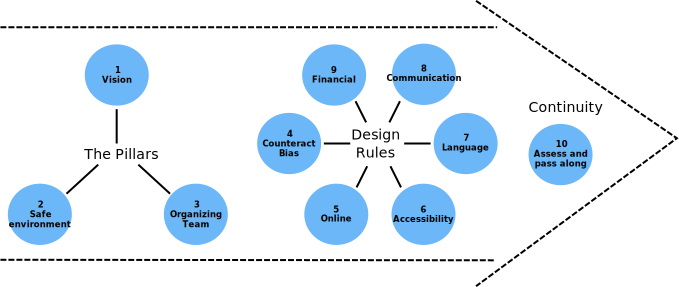
\includegraphics[width=\textwidth]{figs/rules.png}}{
%sara: suggestion for alt text:
%Diagram of how the 10 rules are organized into three groups: grounding rules (rules 1, 2, and 10), people-related rules (rules 3 and 4), and design rules (rules 5 to 9). The diagram has five rows. Each line contains rectangular boxes with the rule number and a short title for each rule. Each rule box is colored based on their group (grounding rules are grey, people-related rules are green and design rules are pink). First row is for the grounding rules 1. Multidimensional diversity and 2. Safe and inclusive environment in grey boxes. Second row is for people-related rules 3. Organizing team and 4. Unbias in green boxes. Third row is for the design rules 5. Online component, 6. Accessibility for disabilities, 7. Language inclusivity in pink boxes. The fourth row is for the design rules 8. Communication and 9. Financial support and budget in pink boxes. The last row is for the grounding rule 10. Diversity and inclusion as a process in grey boxes.
}
\caption{Diagram of the rules organized in three groups: the pillars (rules 1, 2, and 3), design rules (rules 4 to 9), and the process (rule 10).}
\label{fig:diagram}
\end{figure}


\section*{I. The pillars}

To organize a more inclusive conference, it is necessary to identify upfront which groups of people are being excluded, the barriers that keep them from active partaking, and targeted strategies to overcome them. 
\textbf{Rule 1} is about embracing all dimensions of diversity and prioritizing the participation of groups that are often marginalized.
However, increasing diversity alone is not enough. \textbf{Rule 2} focuses on how to create a safe and welcoming environment for all the conference attendees. 
Inclusion should start from the organizing team. \textbf{Rule 3} highlights the importance of starting with an inclusive and diverse organizing team, and provides tips on work dynamics.


\subsection*{Rule 1: Embrace all dimensions of diversity}
\label{rule_diversity}

% Rocío: Main idea: what is diversity and why does it matter? (inequalities)
Diversity encompasses multiple dimensions: age, physical ability, career stage, gender, gender identity, geographic origin, language, neurodiversity, race, religion, sexual orientation, and socioeconomic background, to name a few.
Human diversity should be celebrated and respected in every way. 
Nonetheless, we live in a world with implicit hierarchies along these axes. 
Some statuses (\textit{e.g.}, cisgender, white, male, from North America or Western Europe) hold the privilege of being the defaults around which all systems--including conferences--are consciously and unconsciously built. 
People outside the dominant groups suffer different forms of oppression, like sexism, racism, ableism, homophobia, and transphobia; some people have to deal with several of these on a daily basis.
% While no isolated initiative can drastically alter conference outcomes, building a more diverse and inclusive conference starts by recognizing that these inequalities have systematically excluded whole groups of people from academia and scientific and professional circles. 
Recognizing this systematic exclusion, particularly in our fields and in our scientific or professional communities, will help identify the most marginalized and discriminated subgroups \cite{timperleyHeMoanaPukepuke2020}.
% These are the groups that warrant deliberate efforts that ensure fair inclusion.
As a starting point, identify which groups warrant deliberate efforts to ensure fair inclusion, and determine the contributing factors (e.g. explicit discrimination, participation fees, etc.).
This analysis should guide the vision of diversity and inclusion for your conference and help design strategies to achieve it. 
Express this vision for your conference in a diversity statement. 
Next, use this vision and the set strategies to define measurable indicators and goals of diversity and inclusion (\textit{e.g.}, a gender distribution of your speakers that is representative of the general population, presence of racialized people --especially Black people-- among the head organizers, speakers, and attendees, or participation from key geographic regions). 
These numbers should guide you and help achieve your vision.

% Investing a substantial effort towards the most excluded groups does not mean neglecting the other communities, but will instead ensure equity, guide the vision of diversity for your conference, and help design strategies to achieve it.
% vision
% back to the indicators? 
% realistic but bold (back?)
% be aware and promote awareness
%¡LAS BARRERAS!
%Express the diversity and inclusion vision for your conference by writing a diversity statement. 
% As a starting point, identify which groups are usually unsupported or discriminated against in the community or event of interest, and determine the contributing factors. Next, set measurable indicators of success when organizing a diverse conference. The numbers resulting from these indicators are not the primary goal, and this is not about performative allyship. Instead, these numbers should guide and help hold the organizing team accountable towards these diverse and inclusive goals.

% Rocío: more effort towards including the more excluded
% This may translate into different actions depending on your field, region, or community, \textit{e.g.}, a gender distribution of your speakers that is representative of the general population, presence of racialized people --especially Black people-- among the head organizers, speakers, and attendees, LGBTQIA+ friendly-spaces, or community participation from key geographic regions.


\subsection*{Rule 2: Create a safe and welcoming environment}
\label{rule_inclusion}

% Rocío: main idea: Inclusion for everyone
While it is essential to improve representation towards some of the most visible dimensions of human diversity, such as race, gender, and country of origin, building a truly inclusive environment means taking care of all the other aspects of diversity as well. 
% Edit and make more specific (below)
Promote respect of pronouns, schedule events exclusive for diverse groups (e.g., LGBTQIA+-friendly spaces), and if the conference has an in-person component, set spaces for religious practices, breastfeeding and child care, and include menu options that account for diverse dietary and religious requirements. These are just some examples of decisions that are relatively easy to implement and can have a large impact in making inclusion real (see \cite{noauthor_discover2021} for some great advice on `low-hanging fruits').
Importantly, by being proactive in creating such a welcoming space, you can be respectful of everybody's privacy and avoid requiring anyone to disclose personal information–such as revealing a disability, the sexual orientation, gender identity, or mental health issues, just to a name a few.
% Rocío: Could have a paragraph about active bystandership—Andrea%ö
%promote a supportive and respectful environment where attendants act as active bystanders. y definir '¬¬ 
% Rocío: main idea: Code of conduct for a safe place
Adopting a Code of Conduct and gathering a team to enforce it are key aspects in creating a safe environment during a conference \cite{favaroYourScienceConference2016}.
The Code of Conduct is a document meant to keep the community safe and should state clearly the unacceptable behaviors, the consequences for engaging in such behavior, and the way to report violations \cite{auroraHowRespondCode2019}. 
The Code of Conduct team must receive training on how to receive reports, respond to incidents, communicate their responses, and organize accordingly creating protocols on how to respond. This should be done during the early phases of the conference planning because Code of conduct violations can happen before the conference (e.g. social media, organization meetings).  
Since people from marginalized groups are more likely to be victims of Code of Conduct violations and to see their claims dismissed due to power dynamics, assembling a diverse Code of Conduct team will be essential to deal with discrimination and harassment issues and the power dynamics underneath them and deal with them in a sensitive manner. It may also be more understanding of different disciplinary cultures and geographical and cultural considerations. 
We strongly recommend reading `How to Respond to Code of Conduct Reports' \cite{auroraHowRespondCode2019} as an excellent starting point for the Code of Conduct teamwork.
 


\subsection*{Rule 3: Have an inclusive and diverse organizing team}
\label{rule_organizing_team}

% Rocío: Idea of this paragraph: build a diverse team, and representation

A genuinely inclusive conference can only be organized by an inclusive and diverse organizing team in charge of the conference decision-making.
Organizers should be a team with people from different regions, genders, races and ethnicities, socioeconomic statuses, and other aspects of diversity.
Having diverse people in decision-making positions will positively affect all the other aspects of your conference because all the processes will benefit from their input, expertise, and distinct perspectives \cite{hongGroupsDiverseProblem2004}. 
In addition, a diverse team plays an important role in creating a welcoming space because representation--seeing people with similar life experiences occupy public spaces, positions of power, and breaking negative stereotypes--is one of the best ways to create a sense of belonging for everyone participating in the conference (see Rule 2 about a safe and welcoming environment). If you already started assembling an organizing team, check for gaps in its composition. 
The regional and local communities, groups, or associations in your field are good sources to tap into. 

% Rocío: Idea of this paragraph: non-transferability and do not restrict people
People with disabilities often say: `Nothing about us without us'; the same holds for other dimensions of diversity. This means that the actual life experiences, expertise, and insights from people in marginalized groups cannot be replaced by good intentions from people outside these groups \cite{costanzachockDesign2020}.
People who have experienced exclusion have the social and technical expertise to fight against it and they will be essential in any team.%ast maybe frame this on a more positive note (ideas, problem solving)
However, they must have the freedom to choose in which areas of the conference they want to work and not be restricted to diversity and inclusion aspects. 
% Rocío: Idea of this paragraph: tips to make a diverse and inclusive team work + paying them
When working with people from marginalized groups do not assume that self-nomination and voting will work as mechanisms to choose leadership positions. Instead, nominate directly and offer leading positions that would normally be occupied by people from privileged groups.
Build an environment in which every person can express their opinion and pay special attention to people from systematically excluded groups.
Many people lack the institutional support to put time and effort into the organization tasks and do not have the luxury to commit to the organization for free; consider paying them as an item in your budget.  
% Rocío: Add other types of recognition besides money (website, public recognition on social media, during the conference, etc.)
In addition, tasks such as receiving and responding to Code of Conduct reports can be emotionally intense work and should be additionally rewarded.

% % Rocío: might go to the next rule
% Splitting the workload and responsibilities should not be done by putting care-taking labors--community building, meeting organization and note-taking, conversations with potential partners--on the hands of women and other minoritized groups, while people from privileged groups take the lead in stereotypical highly-valued tasks (see \textbf{Rule \ref{rule_unbias}}). 


\section*{II. Design Rules}

These rules concern diverse elements in the design of the conference and operational tasks. They are all important pieces for inclusion.
In rule 4, we introduce ways to counteract bias in the conference program, in keynotes, program committee, abstract selection, and other spaces. 
Rule 5 describes the advantages of online conferences reducing barriers for participation, and provides advice for organizing online and hybrid conferences.
Rule 6 focuses on practices to make all conference platforms and spaces accessible to people with disabilities. 
In rule 7, we advocate for more language-inclusive conferences, and provide suggestions to encourage and ensure full participation of non-native English speakers. 
Rule 8 provides tips for an inclusive media strategy. 
In rule 9, we address budgeting for inclusive practices, and helping participants with affordable registration costs, scholarships, and other forms of financial support.


\subsection*{Rule 4: Consciously counteract bias in the conference program}
\label{rule_unbias}
%idea of paragraph 1: our lists are biased

When choosing or inviting people for visible and valued roles in the conference––such as keynote speakers, program committee members, session chairs––, it is likely that there will not be much diversity in the first set of names.
Our biased lists are products of the existing systems that have always privileged some groups of people \cite{dwyerNoticeWhoScience2021,swartzScienceValueDiversity2019,wongBuildDiversityScience2020,dignazioUnicornsJanitorsNinjas2020}. 
Rather than deter us, this should encourage us to go beyond our narrow and often limited networks to look for, reach out to, invite, encourage, and onboard great people that are not routinely in the spotlight, making sure that these roles do not stay with people in privileged groups (e.g. avoid `manels' and all-white panels, for instance).
Make sure the composition of all these groups is balanced across topics, areas, and representation across regions, gender, and race.
%rita: For academic conferences consider also to select for a talk master and PhD students and not to give voice only to senior scientist or principal investigator. lo pongo acá porque sí faltan cosas prácticas.


% our committees are biased and unconscious bias exists
%Having a chance to present at a conference is an opportunity to gain--or keep--visibility in the community or field.

The final list of accepted talks can also be biased. 
On the one hand, because people do not feel confident to submit their work. 
To counteract bias in submission, promote your calls beyond the usual communities and keep in touch with local groups and communities of practice to encourage submissions by their members.
Some of these communities have pre-submission mechanisms to help their members prepare and improve their submissions.%sin el ejemplo no se entiende
% 1. Clear rules on reviews: double blind, double open, kind of open, etc.
% Be transparent on the evaluation criteria
% 2. Diverse program committee (above)
% 3. Unconscious bias (test)
% 4. Curate the final list against 
%see: https://www.science.org.au/files/userfiles/support/emcr/documents/one-page-summary-emcr-improving-diversity-web.pdf
On the other hand, proposals may be biased because of even diverse selection committees can be subjected to unconscious or implicit bias %explain!.
Unconscious bias happens when we interpret information, such as names of the authors, we assume their origin or ethnicity, their institution of origin, and we attach a positive or negative value to their work according to negative or positive stereotypes. 
To counteract this...
The review process should guarantee the fair evaluation of the submitted work, and this may  will be double blind, open, or partially open. 
In some fields, it's not possible to guarantee anonymity of the presenters, and in some and external cues such as country of origin and links to repositories. 
Create clear evaluation criteria for the submitted proposals, and share them with the authors and reviewers.
Remind the reviewers that unconscious bias exists and encourage them to take unconscious 
Selection committees need to be reminded of such biases, and be aware of them when evaluating submissions and presentations.
\cite{swartzScienceValueDiversity2019, wongBuildDiversityScience2020}

% Rocío: main idea: unbias roles and give spotlight to the roles--and people who have contributed in roles--that are not stereotypically categorized as success
Activities such as scientific publication and development of software are often regarded as higher value than other roles like community building or teaching. 
These roles may be equally if not more challenging and are usually assumed by women, people of color, people with disabilities, and other minoritized groups \cite{cheng2020x+, burfordHomelinessMeantHaving2020}. Research about these topics is equally undervalued compared to other areas of knowledge production. 
Counteracting bias also means changing the standard program of the conference, proposing new thematic sessions, broadening the scope of talks, keynotes, and tutorials, // and giving visibility to the whole range of activities and practitioners that contribute to the overall topics of the conference. 

%Defy the stereotypical criteria for merit and how it is traditionally measured by acknowledging these community practices and the people behind them.
You can also reframe the awards ceremony to acknowledge work beyond the traditional definition of merit/quality and include those who contributed to community building, presented teaching materials, and assumed other care-taking roles.


\subsection*{Rule 5: Have a strong online component} 
\label{rule_online}

% Rocío: main idea of the paragraph: online conferences can open opportunities for inclusion
%1. in 2021 an inclusive conference has to be an online or hybrid conference. this means a radical change in the functioning of all spaces, to include people who are online for any reason. we have elements to advocate for hybrid and lots of refs about online. cite joo and online refs. 
%practical: choose the platforms and be aware that reach varies between countries. check accessibility. understand bandwidth limitations. online does not make it automatically inclusive.
%2. hybrid. we advocate for active hybrid and distributed hybrid conferences because it's the most inclusive formats (not passive hybrid or semi-passive hybrid). we want all the inclusiveness of the in-person component with the _practical_ adaptations for hybrid (chat platform, q and a, streaming and networking) being online or in-person should not affect the possibility to be a chair a keynote or a presenter. no need to be present. a potential problem: opportunities of networking.
As stated in [the nature correspondence]: The COVID pandemic forced us to embrace online conferences (see C. Woolston Nature 582, 135–136; 2020), which remove some of the barriers that disproportionately affect marginalized groups. These include the cost of registration, transport and accommodation, the logistics of long-distance travel, and discriminatory visa applications (H. J. Niner \& S. N. Wassermann Front. Mar. Sci. 8, 638025; 2021; Gewin, V. Nature 569, 297–299; 2019). Inclusive conferences must have an online component [cite all the other references].
In-person interaction at conferences is priceless but often this is true and possible only for the ones who can afford to attend. 
Barriers such as cost of registration, transport and accommodation, the logistics of long-distance travel, and discriminatory visa applications, are particularly true for conferences that usually take place in high-income countries \cite{arendDisparityConferenceRegistration2019,gewinWhatScientistsShould2019,jooKeepOnlineOption2021}. 
Online conferences are more inclusive because they do not require a visa or a big budget, and are more accessible to people who may be unable to travel because of health issues or family responsibilities \cite{salibaGettingGripsOnline2020}.
This means that online conferences have a greater reach, not only in terms of attendees but in terms of speakers  \cite{atkinsonJournalMedicine20202021, roosOnlineConferencesNew2020, jooKeepOnlineOption2021}.
The online format may also make it easier to be inclusive of geographic regions by encompassing several time zones or deciding to rotate the favored time zone every year, without depending on a conference central location. 

%Saranjeet: About time zones, although we can rotate and have different days dedicated to different time zones, we could also try spreading the conference time to be longer. So that each day the conference runs live for a couple of hours or so and the recorded material is made available/uploaded on YouTube (say) soon (every day). This might help because, not everyone might have the luxury of attending 4-6 hours of the conference on a weekday, even though it is running in their local timezone. However, people might be able to attend a couple of hours even on weekdays and will not get the feeling that they have missed a huge chunk of the conference. 
%ast add something about online giving flexibility in formats and how that depends on to the context of the conference
% Rocío: main idea: Networking may seem the weakest part of online conference, but it doesn't have to be. 
Networking and socializing have been mentioned as challenging aspects of online conferences, mostly because we are used to interactions at in-person social settings such as coffee or lunch breaks \cite{salibaGettingGripsOnline2020, roosOnlineConferencesNew2020}. 
%However, in-person settings might not be comfortable or appealing to everyone for socializing and some of these spaces may be exclusionary (e.g. galas or dinner nights at expensive venues). 
However, there is evidence that virtual communication before face-to-face interaction can make people from minoritized groups feel more included, thus participate more (e.g. \cite{trianaDoesOrderFacetoFace2012,blackEngenderingBelongingThoughtful2020}.
% JPNG: "On the other hand, there is evidence that virtual communication before face-to-face interaction can make people from minoritized groups feel more included, thus participate more (e.g. [29, 30]). Written media like chats create opportunities for long term interactions and networking by allowing more people to join the conversation even when it has started some time ago."
Organizers of online conferences should invest time in creating opportunities to meet and bond virtually, respecting people's limits, preferences, and remembering that `the usual' does not necessarily work for everyone, and that no single networking activity will ever serve the whole community. 
It is worth trying new and varied activities centered around different groups of people outside the mainstream of your conference.
%la: see https://www.trainingforchange.org/wp-content/uploads/2017/11/Mainstream-Margin-in-Groups.pdf
Some ideas in this line are: offering the option of written chat in addition to voice or video conversations, opening events with teamwork like trivia, offer some events that can be enjoyed passively like movies, yoga sessions, or art displays, where attendants can choose to just sit and enjoy without talking, or have a chat channel to comment on their experiences during the session.\fede{another activity: virtual city tours, I had it as a corollary activity for a summer school} \la{Some more specifics on how to achieve these suggestions in this paper: https://osf.io/k3bfn/}
% we need to check if something here (newbies!) is not missing in the above paragraphs
% As we mentioned previously, conference attendees should have ample opportunities to network with each other. However, having a diverse offer of networking opportunities that can appeal to people with different backgrounds, accessibility needs, and preferences can be challenging, especially if you have the mindset of organizing each activity for the complete pool of attendants. If you think of smaller activities that can reach specific groups, preferably co-led by community leaders, these sessions can be more productive successful, and inclusive than trying to organize one single activity that can please the whole community (\textbf{Rule \ref{rule_unbias}}). Some examples are the newbies sessions for first-timers, mixers lead by specific subgroups or communities, or leisure activities that reunite subgroups with the same interests: arts, exercise, sports, movies, etc.



% Rocío: main idea of the paragraph: In the context of reopening, hybrid conferences may be a thing. They also need to be inclusive.
Alternatively, a conference could have a hybrid format with an in-person and an online components that articulate well and maximize the experience of everyone attending your conference. This dual format could allow a group of people to interact face-to-face while providing many others the opportunity to participate remotely. 
Conference organizers who have been holding hybrid events since 2011 [Wenger-Tayner, 2021] consider that inclusive hybrid events are the future. These authors emphasize the need that all participants of hybrid events must go through the same event quality to the point that in-person and online participants pay the same registration amount to participate in high-quality hybrid conferences. These authors recommend having a buddy system, where every person attending online has an in-person attendant that makes sure the online person can follow the event and participate in the event as if they were in the room [Wenger-Trayner, 2020]. Wenger-Trayner (2020, 2021) also recommends having a chat function for back-channel conversations between all attendants, a virtual space for all online attendants to talk to each other, and allocating time to small group conversations, often mixing in-person and online groups. 
% Within the context of the COVID-19 pandemic, many conferences embraced the online format; but at the time of writing, some are reverting to in-person, which risks going back to the barriers mentioned above \cite{jooKeepOnlineOption2021}.
The challenge and requirement for this kind of setting would be to make the online component as relevant as the in-person component and not just a consolation prize to the less privileged in the community \cite{jooKeepOnlineOption2021,ninerBetterWhomLeveling2021}.
\rita{Sessions of an hybrid conference could have both chairs online, as attendee or speaker. This mean that is important when organizing the conference to include a third person who is in the venue to help the in-person participants, take the questions that are both online and in-person and communicate with the remote session chairs.}

\rita{The chat system of the conference can have a list of all the participants, with their registration name and if they are on-line or in-person, to facilitate the connections.}  The physical venue will have to include multiple ways to connect with online folks such as tablets on the meeting venue tables and cameras that allow online attendants to follow who is speaking in the in-person space. 
\rita{The venue selection must respond to some criteria such as give online support both bot in-person and online participants, to have stable and secure connection for the in-person participant to join the online event. Moreover, offer the option to create virtual room to connect in-person and online participant for networking events, such as scientific interest group, or LGBTQIA+-friendly spaces. Exhibition stands in the venue need to have facilities to connect with online participants (virtual stand). Furthermore, the poster session need to be carefully thought to give the best experience to both in-person and online participants. This should have both components to allow online participants to see the poster and have the possibility to ask questions. However, it also need allow who want to present their poster virtually to be seen by in-person participants and respond to questions about their works. Lastly to better plan your hybrid conference ask in advance who wish to travel to the venue and who wish to participate online. This will save you time and money for looking for a suitable venue.}

% [Wenger, 1999] https://doi.org/10.1017/CBO9780511803932
% [Wenger-Trayner, 2020] https://wenger-trayner.com/all/in-person-and-online-events/
% [Wenger-Trayner, 2021] https://wenger-trayner.com/reflections/in-person-online-hybrid-the-future/


\subsection*{Rule 6: Make the conference accessible to people with disabilities}
\label{rule_accessibility}

% Be more direct
Conferences are among the least accessible spaces that people with disabilities may encounter in professional contexts \cite{priceAccessImaginedConstruction2009}. Even when conferences implement other inclusive practices, the participation of people with disabilities is often overlooked \cite{marks2021meeting}. This is one key aspect where participation in the organizing team allows disabled people to take part in the decisions from the beginning (see rule 3 about the organizing team), as thinking about disability or simulating it are not substitutes for real-life experience \cite{costanzachockDesign2020}. Planning for accessibility requires time and early decision-making \cite{irishIncreasingParticipationUsing2020}. As other aspects of inclusion, dealing with accessibility at the last minute is the recipe for a disastrous conference. If you do not consider accessibility from the conference inception, it is highly likely you will be better off without trying to patch accessibility at the last minute. Key decisions in this respect are hard to correct.

For in-person components of conferences, the venue should comply with common accessibility standards, such as being adequate for people who use wheelchairs, have signs in Braille, and a sound system compatible with hearing devices and live interpretation, just to name a few important features. In addition to this, the organizers should take care proactively of invisible disabilities (e.g., dyslexia, anxiety, ADHD, autism and its spectrum). This could be done in many ways, for example, by providing quiet spaces for privacy and noise-free conversations, or providing chairs in open spaces.

Regardless of the conference format, all platforms (website, chat, conference administration tools) and images used for the communication strategy of the conference should be screen-reader friendly and keyboard accessible, and have alternative text. Any videos should have good-quality captions and a transcript.
The organizing team should provide accessibility guidelines for slides and presentations, encourage their use, and be available for any questions presenters and attendees may have. Slide decks should be made available beforehand, either in webpages or available for download to ensure that everybody can follow their content during the presentations. 

Accessibility practices should also include social events and networking, and include activities that do not restrict participation based on body type or ability. Importantly, all these accessibility practices are inclusive not only for people with disabilities but to everyone.
For instance, captions are helpful for non-native speakers, having the material available for download helps attendees with low bandwidth connection, etc. Accessibility efforts should be explicitly displayed in the official communication channels (see rule 8 about communication strategy). 

%Live captioning or interpretation! and surtitles (Rita) LA: provide live, high-quality (automated captions are often referred to as "craptions"), captioning or simultaneous translation in English for persons who only speak English. After all, captions and simultaneous translations are common place in the audiovisual industry and your conference audience will likely be already familiar with this if they ever watched a movie from a non-English speaking country.


\subsection*{Rule 7: Don't let language restrict high-quality participation}
\label{rule_language}

% Rocío: main idea: English as the only language makes some people privileged and is a barrier for others
In international meetings, the linguistic diversity of the participants is often overlooked. 
English is usually the official and sole language for submissions, presentations, tutorials, workshops, conference platforms, webpage, and official communications. 
While English is indeed regarded as the primary language in scientific communication and one official language makes it conducive to communicate widely, this makes being a native English speaker a privilege.
Non-native English speakers could miss opportunities to attend or actively participate in conferences (e.g. asking questions or participating in discussions),
and conferences may in turn miss innovative contributions.


% Rocío: main idea: make conferences more linguistically inclusive
Providing a welcoming and diverse environment by encouraging the full participation of non-native English speakers is critical (rule 2 about a welcoming environment for all). This may be done at different levels. 
For presentations spoken in English, provide English-to-English captions to help non-native English speakers (in addition to people with hearing disabilities) follow the presentations. Whenever possible, identify other key languages for the conference and provide translated captions or live interpretation into these key languages, including multilingual Q \& A sessions.
The following step would be having sessions and events in languages other than English, both regarding the technical content of the conference and the social and networking aspects. Networking sessions in languages other than English can include captions or interpretation or not, which has the benefit of not requiring major technical adjustments. Keynotes and regular talks should always be accompanied by captions or live interpretation to English.

Promote the attendance to presentations in languages other than English as key components of your schedule and announce when captions are available. 
Remind your native English speaking audience to be respectful of accents and mistakes in English from non-native English speakers. 


% Rocío: we could eventually cite https://conferenceinference.wordpress.com/2020/11/30/when-language-is-not-a-barrier-a-tale-fr[…]istically-inclusive-conference-toma-pustelnikovaite/


\subsection*{Rule 8: Express the welcoming spirit in your communication strategy}
% media
\label{rule_communication}

%Rocío: Main idea: Include people in your communication 
The communication strategy of your conference should aim to increase the number and diversity of participants, and be inclusive by design.
Actively reach out and promote the conference to people who have been systematically excluded. 
Publish the diversity statement, the Code of Conduct, the accessibility guidelines, and  options for financial support (see rule 9 about financial resources), to emphasize that everybody is welcome in the event.
Try to come up with creative ways to show that everyone is seen, respected, and welcome. For example, useR! 2021 created a mascot for the conference wearing different scarfs reflecting folks from different groups that the conference wanted to reach (Fig. 2). 
The diverse organizing team should be able to help deciding which languages to emphasize and which social media platforms to utilize in the promotion of the conference (e.g. Twitter, Facebook, LinkedIn, conference website, mailing lists).

%lA: in case it is not mentioned later: If your budget does not allow to accommodate everyone, at a bare minimum, you should inform potential attendant which accommodations you do provide and which you will not. This will help everyone to know up-front what to expect and save their time if your conference does not accomodate their needs adequately.%ast: responsible communication!
%Rocío: Main idea: Use inclusive language
Inclusive language--language free from words, phrases or tones that reflect prejudiced or discriminatory views of particular people or groups--should be used in all communications \cite{hallDesigningDiversityInclusion2019}. 
Make the effort to teach yourself the vocabulary about disabilities, racialized groups, and gender and sexual orientations. %
Do not expect minoritized people to teach you--it's not their role--, and accept feedback without being offended.
Inclusive language also encompasses avoidance of excessive and too specific technical jargon and acronyms. 
%
% links, examples, this changes with the context
%practice: create a standards in inclusive language for your community, to build collective knowledge than can be passed to 

% Rocío: could add some ideas from here 
% https://www.science.org.au/files/userfiles/support/emcr/documents/one-page-summary-emcr-improving-diversity-web.pdf

\begin{figure}[!h]
\centering
\pdftooltip{
\includegraphics[width=\textwidth]{figs/marmots.pdf}}{
}
\caption{Margot the marmot was useR! 2021 mascot}
\label{fig:marmots}
\end{figure}

\subsection*{Rule 9: Allocate adequate financial resources to support your conference goals}
\label{rule_financial}

% Rocío: main idea: Budgets are limited and need to choose priorities.
Allocation of resources to support the goals of inclusion of the conference has to be intentional. 
Estimate the costs for these practices and define your priorities in advance (e.g. paying the organizing team, Code of Conduct training, captioning).
Additional support for attendees could also be considered in the budget: child care support, transportation fees, visa-related support (if in-person), internet connection services (for the virtual component). 
Consider that an online conference might reduce organization costs (e.g. no rental costs for a physical venue), allowing to redirect the money towards other inclusive priorities. 
When asking for sponsorship, it might be easier to justify supporting concrete actions towards inclusion than making generic demands for funding.

% Conference budgets are limited and rely mostly on sponsorship and attendance fees. 

% Rocío: main idea: help take the burden out of participants for more inclusive participation
When determining the registration rates, the socioeconomic context of participants, their country of origin, and their career status should be taken into account  \cite{sarabipourChangingScientificMeetings2021, andalibPostdocQueueLabour2018, kaplanPostdocNot2012}
(see \cite{canelon2021cost} for an example of conversion rates based on country of origin and career status). 
%In general, people should have the option to locate themselves in a category they consider affordable, even with the possibility of a `pay what you can' approach. 
Resources permitting, allow the possibility of a `pay what you can' option. You could also aim to have a conference with no registration costs; this is especially true for online events, but bear in mind that free events have a lower attendance rate than non-free events \cite{eventbrite_ultimate_2017}. 
%Other costs can be prohibitive-> scholarships
Scholarships to attend the in-person component of the conference are an additional way to boost participation of people from marginalized groups, by offering support for travel and lodging expenses.
Design the diversity-related scholarship to be explicit about the groups you want to support, and be transparent about the criteria for evaluation to avoid self-selection (the fact that some people refrain from applying because they think they don't stand a chance). 
Conferences usually ask for cover letters or applications to assign these scholarships, and this can be a time-consuming, emotionally-demanding task. 
Simplify as much as you can the process of asking for financial support; 
people who do not have the time (e.g., because they have family responsibilities) might decide not to apply if the process is overtly complicated. 
Bear in mind that transferring money internationally is a cumbersome administrative process that can significantly augment the burden of already marginalized groups. Whenever possible, facilitate ways around money transfer (e.g., book flights, hotel reservations, waive conference fees).



\section*{III. The Process}

A conference can make a difference in the path towards inclusion/Conferences are powerful community-building spaces, that can foster change in future events and the community itself. The organizers of a conference edition and selection committees should do their best to pass their knowledge on best practices and problems encountered to future organizers.


\subsection*{Rule 10: Make the conference part of a long-term process for inclusion}
\label{rule_process}

% Rocío: main idea: no first attempt is guaranteed to succeed
Assess whether equity and inclusion goals were met during the conference. 
Part of it can be done internally by evaluating the diversity indicators you defined at the beginning of the planning process. % examples
 
% Ask for feedback to know the extent of your success
Ask for feedback about the conference experience of the participants by posting a survey during and after the conference. 
Make open answer options to let people self-identify and express their opinions freely. Let all responses be optional and anonymous and commit to confidentiality and data privacy. 
The survey results will allow you to identify the aspects that worked towards your inclusion goals, and understand what went wrong and how people were excluded.
Do not expect everything to be perfectly inclusive, or to encompass all the dimensions of diversity at once. %You're part of a process and contributing to structural change.

% Pass the information
Document your processes, lessons, and guides in blog posts, reports, and presentations. 
Facilitate contacts with the people you worked with along the process. 
Make sure to share this information with future organizers,
they will have a starting point and their work to improve inclusion in the following editions of the conference will be easier.
If you are part of a stable meetings committee, encourage organizers to follow these rules and advocate for setting up new standards for inclusion. 
%hablar del pasado - shoulder of people before, federico
%sale? Most importantly, there are systemic discrimination issues at higher levels (e.g. society, academia) that one conference cannot change. 
%\la{Due to these systemic problems, even the minimum changes to how conferences have been historically organized will find resistance}, but your courage to make changes will be a step towards a more diverse and inclusive community, and can have a huge impact in the lives and careers of often excluded and minoritized people.



\section*{Concluding remarks}

This article suggests changes in conference planning towards diversity and inclusion to make them networking and learning opportunities for all. 
Organizing a conference and implementing inclusive practices are both learning experiences;
you may not achieve everything you aimed for, set priorities and remember rule 10: diversity and inclusion are processes. 
Most importantly, there are systemic discrimination issues at higher levels (e.g. society, academia) that a single conference cannot change. 
Due to these systemic problems, even the minimum changes to how conferences have been historically organized may find resistance, but your courage to make these changes will be a step towards a more diverse and inclusive community, and can have a huge impact in the lives and careers of people who are often excluded.
Moreover, if more conferences and domains apply these rules, there will be less resistance, the process will get more streamlined, straightforward, and mainstream to adapt with minimal overhead.
% Rocío: I don't like the ending.
(Guidelines/documentation) may be useful not only for your conference series but also for other communities with the same questions that you have. % Give examples of how others have helped us.

\section*{Acknowledgments}
The authors of this piece would like to thank every single member of the organizing team of useR! 2021 [ \url{https://user2021.r-project.org/about/global-team/}] for their valuable contribution to an inclusive conference experience, and the R Foundation for trusting us with the organization of useR! 2021 and supporting us through the process. 


% \nolinenumbers

% % Either type in your references using
% % \begin{thebibliography}{}
% % \bibitem{}
% % Text
% % \end{thebibliography}
% %
% % or
% %
% % Compile your BiBTeX database using our plos2015.bst
\bibliography{community-science}
% % style file and paste the contents of your .bbl file
% % here. See http://journals.plos.org/plosone/s/latex for 
% % step-by-step instructions.
% % % 
% \begin{thebibliography}{10}

% \bibitem{bib1}
% Conant GC, Wolfe KH.
% \newblock {{T}urning a hobby into a job: how duplicated genes find new
%   functions}.
% \newblock Nat Rev Genet. 2008 Dec;9(12):938--950.

% \bibitem{bib2}
% Ohno S.
% \newblock Evolution by gene duplication.
% \newblock London: George Alien \& Unwin Ltd. Berlin, Heidelberg and New York:
%   Springer-Verlag.; 1970.

% \bibitem{bib3}
% Magwire MM, Bayer F, Webster CL, Cao C, Jiggins FM.
% \newblock {{S}uccessive increases in the resistance of {D}rosophila to viral
%   infection through a transposon insertion followed by a {D}uplication}.
% \newblock PLoS Genet. 2011 Oct;7(10):e1002337.

% \end{thebibliography}



\end{document}

